Space exploration is a fast-moving field, with engineering advancements driving a move towards precise and efficient landing systems. Landing systems are critical to enabling cost-effective launches of satellites and human space exploration. Blue Origin and SpaceX have developed reusable rockets like the New Shepard 4 and Falcon 9 to reduce space access costs. These rockets require precision landing of different degrees to land on a fixed launch pad or autonomous drone ships. The most advanced rocket is Space X's starship, which has to hover accurately a few 10s of meters above ground before being caught by metal claws, as shown in \autoref{fig:starship_catch}. NASA's Artemis program and SpaceX's ambitions extend these mission requirements to the Moon and Mars.

\begin{figure}[H]
    \centering
    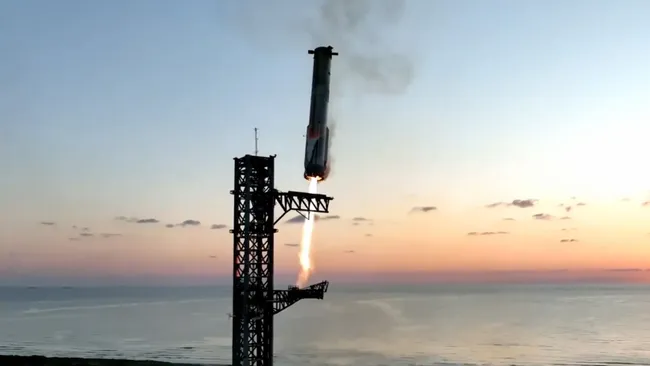
\includegraphics[width=0.95\linewidth]{figures/LiteratureStudy/StarshipCatch.jpg}
    \caption{Starship catch. Image credit: SpaceX.$^{0}$.\label{fig:starship_catch}}
\end{figure}
\footnotetext{\url{https://www.space.com/spacex-starship-super-heavy-chopsticks-catch-near-abort} (Accessed: 04-12-2024)}

To land the rocket, precision and robust control systems are required, containing sensors, actuators and control algorithms. To understand the traditional mechanisms and algorithms used, first RETALT1's Guidance, Navigation and Control (GNC) system is reviewed and applied to our problem in \autoref{sec:GNC}. The RETALT1 project was a European Union Horizon program initiative to advance the research and development into technologies needed for for vertical landing launch vehicles. Following this, the different flight phases a two stage launch vehicle covers during ascent and landing are reviewed in \autoref{sec:flight_phases} focusing on the RETALT1 description and real-World results from Space X's \textit{Starship} launch vehicle.

Finally, current high-level trajectory optimisation methods are reviewed of loss-less convex optimisation (\cite{Acikmese2007}, \cite{Acikmese2013}, \cite{Blackmore2010} and \cite{Wang2020}) and Model Predictive Control (MPC) (\cite{Wang2018}), in \autoref{sec:convex_optimisation} and \autoref{sec:MPC} respectively. Trajectory optimisation is an important part of landing as it ensures a safe and accurate landing, while minimising fuel consumption. However, traditional methods are shown to be computationally complex, which can limit their real-time application effectiveness, causing a trade-off between solution optimality and real-time feasibility. Advances in machine learning in the field of deep reinforcement learning were neural networks are used as function approximators how provided a potential solution independent of the trade-off. Deep reinforcement learning (DRL) in terms of applications to the rocket landing problem are presented in \autoref{sec:DRL}.

\subsection{Guidance, Navigation and Control architecture}
\label{sec:GNC}

RETALT1's GNC system takes in sensor readings and a reference trajectory to provide actuator commands. First the \textbf{flight manager} sets the flight phase, for example vertical rising or boostback burn. Then, the \textbf{navigation module} takes in sensor readings and adjusts them when required through techniques like filtering or state estimation to estimate the state of the rocket. With the flight phase given from the flight manager, the estimated state from the navigation model and the reference profile already generated the \textbf{guidance module} provides a reference attitude and actuation commands to the \textbf{control module}, using feedback to augment its outputs (control reference). Finally, the \textbf{control module} actuators the actuators. This process is shown clearly in \autoref{fig:GNC_architecture}.

This provides a modular architecture, which data-driven control methods could unify into a smaller framework providing a GNC system with less complexity and smoother flight phase transitions. On the other hand, data-driven methods could also replace individual blocks like Guidance and Control, acting as an end-to-end controller, or generate an optimal reference trajectory and optimise the switching conditions in the flight manager. In summary, data-driven methods could increase the performance RETALT1's GNC system in different ways.

To better understand the state of the vehicle one can have without complex state-estimation techniques, the sensors are looked at. These are listed below, and the total observable state space is created in \autoref{eq:total_obs}; this can be used with the control system design to use the observable states as feedback. Mass states are added as the mass used can be estimated through throttle commands.
\begin{itemize}
    \item Inertial Measure Unit (IMS): measures acceleration and angular velocity through gyroscopes and accelerometers.
    \item Global Navigation Satellite System (GNSS): provides the rocket's position, but on Mars is unavailable as there are no satellites in orbit there which perform GNSS requirements.
    \item Differential Global Positioning System (DGPS): is similar to GNSS, but provides more accurate position information through a ground-based correction.
    \item Flush Air Data System (FADS): measures aerodynamic parameters like dynamic pressure, static pressure, angle of attack, side-slip angle and Mach number.
    \item Altimeter: measures altitude.
\end{itemize}

\begin{equation}
    \mathbf{o} = \bigg[ \underbrace{\{x, y, z, h\}}_{\text{Position}}, \underbrace{\{\vec{v}, \vec{a}\}}_{\text{Linear states}}, \underbrace{\{q_0, q_1, q_2, q_3\}}_{\text{Quaternions}}, \underbrace{\{\omega_x, \omega_y, \omega_z\}}_{\text{Angular velocities}}, 
    \underbrace{\alpha, \theta, \gamma, \beta}_{\text{Angles}}, \underbrace{\rho, M, p_a}_{\text{Aerodynamics}}, \underbrace{m_{\text{prop}}, m}_{\text{Masses}}\bigg]
\label{eq:total_obs}
\end{equation}

To control the rocket actuators must be able to provide forces and moments in each axis. First, each thruster has a main valve to initiate or shut-down the thruster. Second, for a full-flow staged combustion cycle, where the propellants are gasified in pre-burners which are used to drive turbopumps in main combustion chamber, the turbopump's rpm is altered to throttle the engines. Throttling is needed during ascent to avoid the rocket reaching maximum dynamic pressure, likewise in landing, but along with providing precise velocity control.

To adjust the flight path of the rocket to allow it to flow a curved mission profile, torque is needed to rotate the rocket, for the thrusters the Thrust Vector Control (TVC) system performs this (\cite{sutton_rocket_2016}). A gimballed pivot TVC system is chosen for this case study, as it is a "simple, proven technology" (\cite{sutton_rocket_2016}) and used upon Space X's rockets.

However, during periods of propulsive free flight or otherwise called "\textit{ballistic arcs}" an actuator capable of attitude control without ignited thrusters is required. Two systems are used, first Aerodynamic Control Surfaces (ACS) are used in the denser atmosphere as they effectiveness is linearly dependent to dynamic pressure, and the Reaction Control System (RCS) for the upper atmosphere.

The RCS provides small $\Delta v$ and orientation corrections in the upper atmosphere, but as mainly used for rotation maneuver's it is called a attitude control system (\cite{sutton_rocket_2016}). The actuation side of RCS has most of the moment provide by cold-gas thruster pairs in each axis at the top and bottom of the rocket, where the moment arm is greatest. Due to the "pair" nature of the actuators they can provide a pure moment without forces. Reaction wheels can also be used for fine control without propellant consumption, but only thrusters are considered here as they provide a larger moment. Not that, Space X don't carry propellant for them, but instead use excess ullage gas. Ullage gas is an inert non-combustible gas, like gaseous nitrogen ($N_2$) used to pressurise propellant tanks

The ACS can take several forms, considering only dynamic actuators used in industry. Super Heavy, the first stage of Space X's launch vehicle \textit{Starship} has 4 electrically actuated grid fins (\autoref{fig:gridfins}), which contain a lattice of small aerodynamic control surfaces within the fin. Mounted at the top of the first stage there is a large moment arm allowing for heavy attitude control, secondly they provide aerodynamic drag to the vehicle. Starship, the second stage of it's namesake, uses a pair of flaps at the top of bottom to control orientation allowing Starship to perform a near-horizontal "\textit{bellyflop}" landing for maximum drag.

The \textit{bellyflop} maneuver optimises landing fuel efficiency and manages re-entry forces. After re-entering Earth's denser atmosphere, Starship will re-orientate horizontally as in \autoref{fig:bellyflop}, significantly reducing drag and terminal velocity, while distributing heating loads across the vehicles stables. At around 500 metres above ground Starship's sea-level optimised Raptor engines reignite and the rear flaps fold inward to cause a rapid flip to vertical orientation. Asides from Space X, New Glenn, Blue Origin's re-usable launcher, uses 4 adjustable fins at the top of it's upper stage for aerodynamic orientation control.

\begin{figure}[H]
    \centering
    \begin{subfigure}[t]{0.48\linewidth}
        \centering
        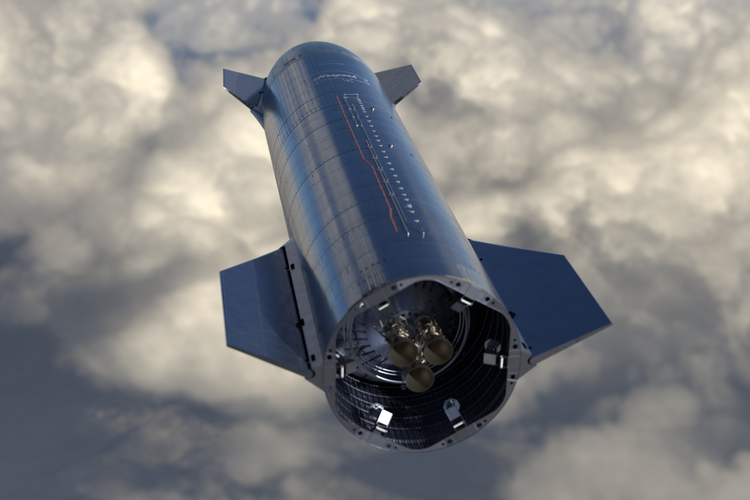
\includegraphics[width=\linewidth]{figures/LiteratureStudy/BellyFlop.png}
        \caption{Starship's orientation during bellyflop.}
        \label{fig:bellyflop}
    \end{subfigure}
    \hfill
    \begin{subfigure}[t]{0.48\linewidth}
        \centering
        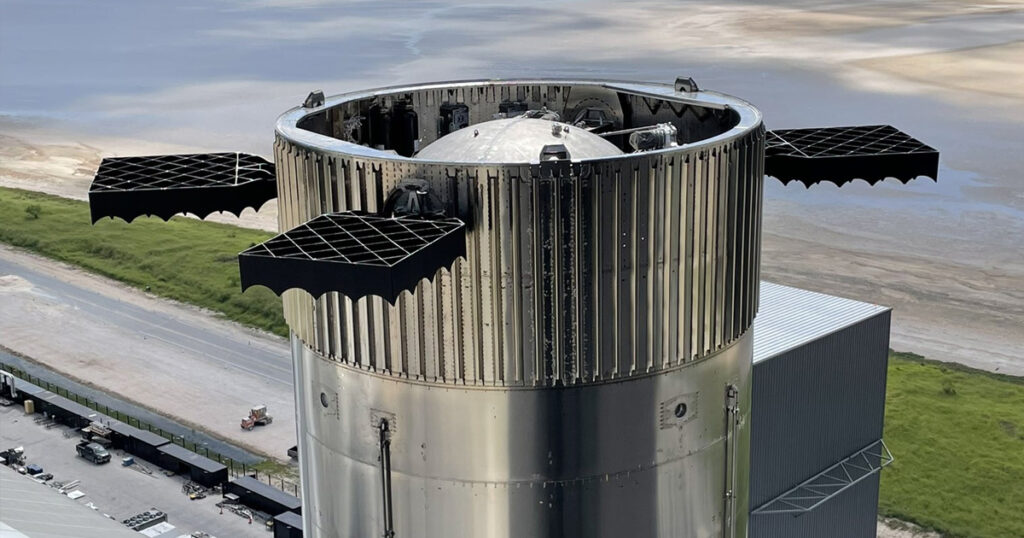
\includegraphics[width=\linewidth]{figures/LiteratureStudy/gridfin.jpg}
        \caption{Super Heavy's grid fins. (Credit: SpaceX)}
        \label{fig:gridfins}
    \end{subfigure}
    \caption{Aerodynamic control surfaces used by SpaceX vehicles.}\footnotetext{\url{https://www.thomasnet.com/insights/spacex-testing-starship-sn8-s-belly-flop-maneuver/}. Accessed on 18-05-2025.}
\end{figure}

Using Space X's Starship launch vehicle as reference, the total available action space can be constructed. This is shown below, with the RCS simplified to only a moment command.
\begin{itemize}
    \item Super Heavy contains 20 fixed perimeter engines, 13 gimballed engines, cold-gas thrusters for reaction control and four grid fins.
    \item Starship has 3 fixed vacuum optimised engines, and 3 gimballed sea-level optimised engines used for the landing burn. Also, there are pairs of fins at the top and bottom of the stage, along with a RCS.
\end{itemize}

\begin{equation}
    \mathbf{a}_{\text{superheavy}} = \bigg[\underbrace{\{\tau_i, MVM_i\}^{33}_{i=1}}_{\text{Throttle}}, 
    \underbrace{\{\theta_i^g, \psi_i^g\}^{13}_{i=1}}_{\text{Gimbal}},
    \underbrace{M_{RCS}}_{\text{RCS}}, \underbrace{\{\theta^{gf}_i, \psi^{gf}_i\}_{i=1}^{4}}_{\text{Grid Fins}}
    \bigg]
\label{eq:super_heavy_actuators}
\end{equation}

\begin{equation}
    \mathbf{a}_{\text{starship}} = 
    \bigg[
    \underbrace{\{\tau_i, MVM_i\}^{6}_{i=1}}_{\text{Throttle}},
    \underbrace{\{\theta_i^g, \psi_i^g\}^{3}_{i=1}}_{\text{Gimbal}},
    \underbrace{M_{RCS}}_{\text{RCS}}, \underbrace{\{\theta^{gf}_i\}_{i=1}^2}_{\text{Grid Fins}}\bigg]
\end{equation}

The action space can be simplified for our problem, for explain not considering roll control, removing the gimbal and grid fin angle in this direction, and reducing the number of controllable grid fins to 2. Also, for different flight phases, different actuators will be used and the others can be unconsidered, set by the flight manager along with the MVM. Finally, the gimbal and throttle commands can be uniform across each gimballed or non-gimballed thruster for a problem complexity reduction, this will reduce the time needed to learn a policy. A more complex control allocation network can be trained in further work taking into account each thruster individually.

The available action space in the reduced form for the problem is \autoref{eq:super_heavy_actuators_reduced} for the first stage and \autoref{eq:starship_actuators_reduced} for the second.

\begin{equation}
    \mathbf{a}_{\text{superheavy}} = \bigg[\tau, \theta^g, M_{RCS}, \theta^{gf}_{left}, \theta^{gf}_{right}\bigg]
\label{eq:super_heavy_actuators_reduced}
\end{equation}

\begin{equation}
    \mathbf{a}_{\text{starship}} = 
    \bigg[\tau, \theta^g, M_{RCS}, \theta^{flap}_{upper}, \theta^{flap}_{lower}\bigg]
\label{eq:starship_actuators_reduced}
\end{equation}

\begin{figure}[H]
    \centering
    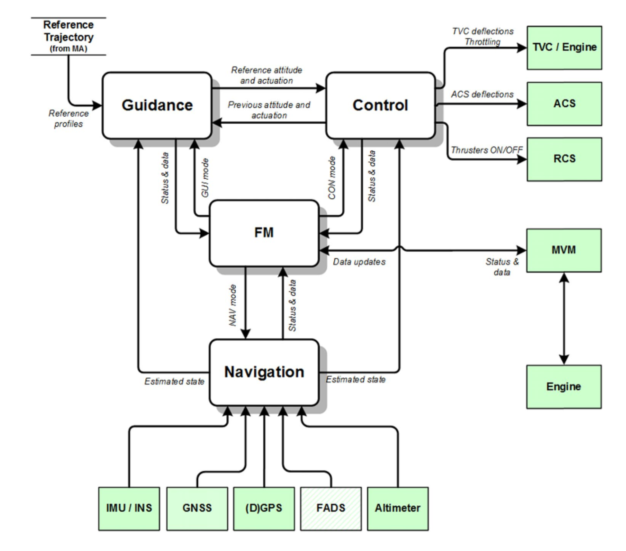
\includegraphics[width=0.95\linewidth]{figures/LiteratureStudy/GNC_architecture.png}
    \caption{RETALT1 rocket's GNC architecture for recovery (\cite{Botelho2022})}
    \label{fig:GNC_architecture}
\end{figure}

\subsection{Flight phases}
\label{sec:flight_phases}

As spoken of in the previous section, the launcher has various flight phases, these are periods of fields characterised by specific aims and atmospheric conditions.  For a two stage launch vehicle the launch starts with a \textbf{vertical rising} phase where the launcher travels vertically upwards to clear the launch tower, before the rocket performs a pitch over (\cite{Launcher_Trajectory}) called a \textbf{gravity turn} to build the horizontal velocity required for orbital insertion. The gravity turn may have to throttle the engines to avoid the launcher's maximum dynamic pressure being breached in the denser atmosphere layers. High dynamic pressure also causes greater aerodynamic forces, a low angle of attack is desired to reduce aerodynamic disturbances.

After the first stage ascent burn, stage separation will occur. In \textit{cold-staging} the fairing between the stages separate and both stages coast for a few seconds, before the second stage's engines ignite. However, Starship performs \textit{hot-staging} to ignite the second stage's engines before fairing separation. This is beneficial as it reduces gravity losses and can provide the first stage with a pitch moment to assist the flip-over manoeuvrer.

After separation, the second stage performs a burn to direct it to orbit using TVC to curve it's thrust vector and the RCS to counteract the minor angular disturbances. Following the burn, it will coast to its orbital altitude before a circularisation burn occurs. Trajectory optimisation for this "exo-atmospheric burn" may use Pontryaigin's Maximum principle to compute the thruster vector and burn time.

Meanwhile, after separation the first stage begins its landing procedure by performing a \textbf{flip over manoeuvrer} to rotate the rocket to near horizontal for a \textbf{boostback burn} to cancel the horizontal velocity. The TVC performs the flip-over manoeuvrer on a limited number of the gimballed engines, which are then fired at maximum throttle to perform the boostback burn, which cuts off the engines once a terminal horizontal velocity has been reached.

The direction of the flip over manoeuvrer depends on the landing scenario, \autoref{fig:RETALT1_flightplant} depicts these two scenarios, with scenario A showing  Return To Launch Site (RTLS) and B showing Away From Launch Site (AFLS) landings. For Space X, AFLS landings the rocket's first stage on an autonomous drone-ship downrange, and RTLS back at a landing pad near the origin launch site.

Trading off, RTLS has lower operational costs and is logistical simpler as no drone ship needs to be deployed for recover, also resulting in a faster refurbishment time as the booster is closer to the processing facilities. Secondly, there is less weather dependence as ocean conditions affect the feasibility of a AFLS landing occurring successfully. However, AFLS recovers less fuel as the boostback burn needs to remove less of the horizontal velocity and thus allows for increased payload capacity. For this scenario, RTLS will be considered do to it allowing for rapid re-usability, one of the main motivations for reusable rockets.

A \textbf{high-altitude ballistic arc} takes place after the flip over, the control authority for orientation comes from the RCS as the rocket is flying through the upper atmosphere, ACS can also assist, but in this problem is not considered.

As the rocket descends into the denser atmosphere the dynamic pressure will increase through increasing density and vertical speed. A burn then occurs to slow the rocket down to avoid dynamic pressure limits and decelerate for landing. Also, with higher dynamic pressure the ACS becomes more effective than the RCS and is used for orientation control.

For Space X's super heavy booster this burn is called the \textbf{landing burn} and the engines burn continually untill landing. However, for some mission scenairos, like RETALT1's mission profile presented in \autoref{fig:RETALT1_flightplant}, the burn is split into two burn with a \textbf{re-entry burn} to avoid the dynamic pressure limits followed by a aerodynamic phase where the ACS maneuvers the rocket, before a final \textbf{landing burn}. Space X's Super Heavy booster profile is selected as it is real-World proven.

\begin{figure}[H]
    \centering
    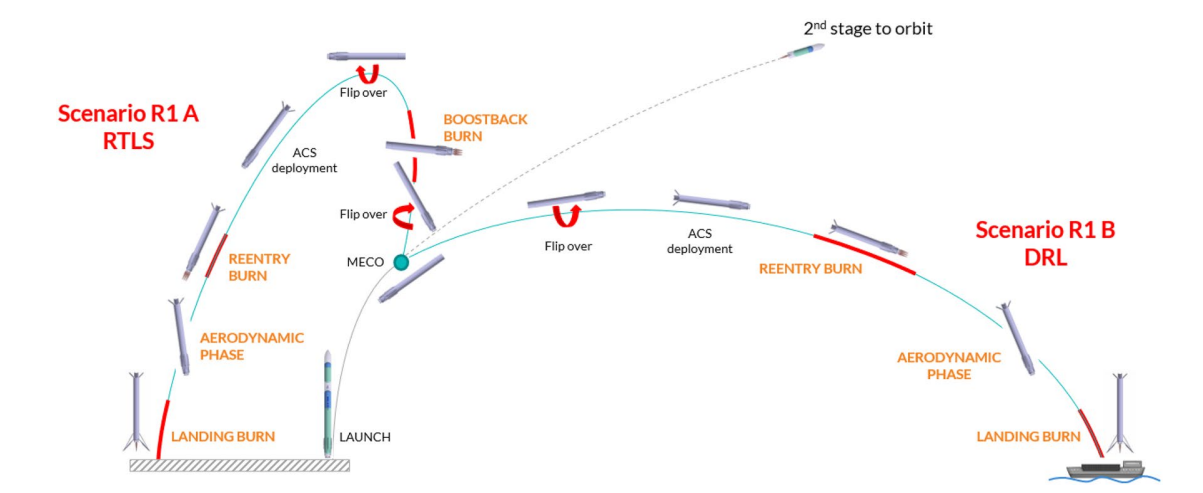
\includegraphics[width=0.95\linewidth]{figures/LiteratureStudy/RETALT1landing.png}
    \caption{RETALT1 return mission concept (\cite{dezaiacomo2022retalt})}
    \label{fig:RETALT1_flightplant}
\end{figure}

\subsection{Descent trajectory optimisation methods}
\label{sec:traj_obj_descent}

Optimal descent trajectory generation for a rocket involves balancing competing objectives leading to a multiple objective optimisation problem (MOOP). First, this MOOP aims to minimise fuel consumption while providing feasibility to the solution. Secondly, the solution must manage strict constraints throughout flight on variables like dynamic pressure and also terminal conditions at the landing site. Several optimisation frameworks have been used specifically for the rocket landing problem, each with differing solution optimality, robustness and computational requirements.

This section reviews three key approaches found in literature, first Model Predictive Control (MPC) which provides an optimal solution and updates with feedback to balance trajectory deviation and actuator usage, allowing for fuel consumption to be minimised. Secondly, the widely applied lossless convexification for rocket landing which provides reliable and efficient solutions but is computationally complex. Finally, a Deep Reinforcement Learning (DRL) approach is presented with the author's (Gaudet) argumentation as to why reinforcement learning is a valid choice.

\subsubsection{Model Predictive Control}
\label{sec:MPC}

MPC is from the optimal control family and uses constrained optimisation at each time step. Given the current state, the future states can be predicted over a finite horizon through the predicted control inputs (\cite{rawlings2017mpc}). The cost function of \autoref{eq:MPC} is minimised to determine optimal inputs, while the states and inputs can be constrained for feasibility. Here $Q$ and $R$ acts as cost weights for state deviation and control effort, setting the costs of state errors and actuation.

\begin{equation}
    J = \sum_{k=0}^{N-1} [(\mathbf{x}_{t+k} - \mathbf{x}_{\text{ref}})^T \cdot Q \cdot (\mathbf{x}_{t+k} - \mathbf{x}_{\text{ref}}) + \mathbf{u}_{t+k}^T \cdot R \cdot \mathbf{u}_{t+k}]
\label{eq:MPC}
\end{equation}

\begin{figure}[H]
    \centering
    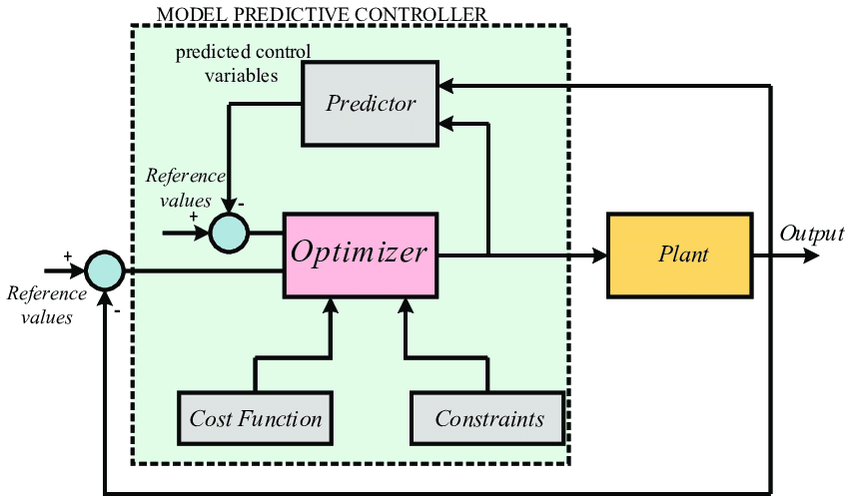
\includegraphics[width=0.95\linewidth]{figures/LiteratureStudy/MPC.png}
    \caption{A schematic of how an MPC works (\cite{Sohaib2018MPC}).}
    \label{fig:MPC}
\end{figure}

\cite{Wang2018} introduce convex-MPC for rocket landing. Stating how it solves optimisation problems while satisfying constraints. In terms of rocket landing it is constrained by dynamic pressure, landing conditions and thermal heating, and has to optimise for minimal fuel consumption. For Wang's convex MPC method the system is repeatedly linearised and non-convex constraints convexified such that convex optimiser used. Furthermore, the MPC optimises the minimisation of the usage of tracking error controls.

MPC is a nice fit for the rocket landing problem due to its ability to adapt to uncertainties in real-time as a finite-horizon optimisation problem. Secondly, it ensures optimal performance under constraints by minimising the tracking error and control effort. However, the finite-time horizon can affect it's long-term trajectory planning, leading to a trade-off between computation time and solution optimality.

\subsubsection{Lossless Convex Optimisation}
\label{sec:convex_optimisation}

% Loss-Less convexification

\cite{Acikmese2007} and \cite{Acikmese2013} use loss-less convexification on the concave rocket landing problem in the Mars environment, where the minimum thrust and thrust vector direction is convexified so that the optimal solution of the convex problem is the same as the concave problem. A lossless solution occurs when the relaxed convex problem's solution is equivalent in optimality to that of the nonconvex problems. \cite{Gaudet2018}, say that the benefit of convexification is that interior point solution methods can guarantee solutions within a bounded time.

\cite{Acikmese2007} start by describing the point mass model of their rocket; here, they assume all thrusters are identical and have the same cant angles, with the position and velocity as the decision variables. The objective is to minimise fuel consumption, which is equivalent to thrust minimisation. A simple introduction introduction of a slack variable on a nonconvex thrust constraint \(T_{\text{min}} \leq ||T(t)|| \leq T_2, \forall t \in [0, t_f]\). This allows the problem to be formulated as a Second Order Cone Programming (SOCP) problem. The constraints are convexified and formulated as a SOCP problem, then discretised into a finite-dimensional problem so optimisation solvers can handle it. This approximates the control inputs as a linear combination of basis functions.

\textit{Lemma. SOCP} (\cite{boyd2003socp})
A class of convex optimisation problems with constraints including second-order (Lorentz) cones. This is shown in \autoref{eq:SOCP}. Note that the variables used here are not in the nomenclature. f is the cost weighting, x the decision variables, m the number of constraints, and A, b, c, d, F, g constraint parameters. 

\begin{equation}
\begin{aligned}
    \text{minimise:}& f^T \cdot x \\
    \text{subject to:}& ||A_i \cdot x + b_i||_2 \leq c_i^T + d_i, i = 1, ..., m \\
    & F \cdot x = g \\
\end{aligned}
\label{eq:SOCP}
\end{equation}

\cite{Blackmore2010} focus on a minimum landing-error approach to Mars landings, aiming to minimise the final distance to the landing site when there is no feasible trajectory due to constraints. First, the algorithm assumes it is feasible and solves similar problems above; if found infeasible, a new trajectory is found to minimise landing error. \cite{Acikmese2013}, take the approaches of \cite{Acikmese2007} and \cite{Blackmore2010}, bring them together and extend them for thrust pointing constraints (cant angle). \cite{mao2017successive} introduces the Successive Convexification (SCvx) algorithm to solve this planetary landing problem with collision avoidance constraints. This algorithm iteratively convexifies the problem before using a "\textit{project-and-linearise}" procedure to transfer the non-convex constraints (state and dynamic) to convex approximations; they argue this allows for a sequence of simpler convex problems to be solved. In more detail, the current solution is iteratively projected onto the feasible set from the non-convex constraints before being linearised around the constraints. Finally, it converges in fewer iterations

% 6 Dof Quaternion problem

\cite{Szmuk_2018} extend the problem to include landing time as an optimisation problem in this 6 DoF form, using the SCvx for linearisation and discretisation into a real-time solvable SOCP problem. Furthermore, trust regions ensure the boundedness of the solution during iterations, and a virtual control avoids infeasibility from poor initial guesses. Finally, further papers with Beh\c{c}et A\c{c}\'{i}kme\c{s}e extend this algorithm with more constraints.

\cite{shen2022realtime} combine convex optimisation with deep neural networks to generate their initial guesses; this reduces computational demands to a 40.8\% reduction in computational time with 99.1\% of test cases reaching real-time requirements. This offers a proof-of-concept of the use of data-driven control techniques to imitate the optimal behaviours of a convex optimiser, albite only for the initial condition and not over the whole trajectory.

\subsubsection{Deep Reinforcement Learning}
\label{sec:DRL}

\cite{Gaudet2018} use deep reinforcement learning to solve the rocket landing problem. They argue that the need for the controller to have stability guarantees is not applicable for rocket landing, as for optimal, linear and Lyapunov (MPC) control, they can only guarantee this with an accurate and validated model, which is hard to get for a complex problem like this, they explicitly state hypersonic re-entry as the example.

Secondly, constrained policy optimisation satisfies the need for hard constraints, clipping the action so it is constrained or even modifying the reward function. Furthermore, it has the additional benefits of allowing for an integrated control (GNC) system and can compensate for sensor noise or offsets. The result was a solution to the Mars-powered descent landing problem, which was robust to parameter uncertainty and noise, on 3 and 6 DoF models.